\chapter{Results}

This chapter presents the results of the analysis performed using the framework.It is divided into two parts: the first presents a comparison of the performance of the three routing metrics, in terms of overall resulting throughput in the network; the second discusses how well each metric would scale to larger topologies than it is possible to use in these experiments.

\section{Comparison of Routing Metrics}
POINTS

hard to distinguish efficient routing metrics on small topologies like pentagon

apparently performs well as flows approach 

limited to 9 Mbps flows
needed to increase offered load, so switched to flow pattern random
RC performance tails off dramatically
unclear why
suspect that it is because the module is unable to find an optimal solution
though there is some variation due to the random the effect is consistent across 15 trials, taken in three blocks of 5 at different times
unclear whether it is significant that flows drop off around 80?


\begin{landscape}
\begin{figure}
\centering
\documentclass[preview=false]{standalone}

\usepackage{color}
\usepackage{tikz}
\usepackage{pgfplots}
\definecolor{mcfblue}{rgb}{0,0.8,1}
\definecolor{mcforange}{rgb}{1,0.6,0}
\definecolor{mcfgreen}{rgb}{.68,.81,0}
\definecolor{mcfgrey}{gray}{0.95}
\definecolor{mcforange2}{rgb}{1,0.8,0}
\definecolor{mcforange3}{rgb}{1,0.2,0}

\begin{document}

\begin{tikzpicture}
  \begin{axis}[
    width = 20cm,
    height = 10cm,
    xlabel = Aggregate offered load (Mbps),
    ylabel = Mean aggregate throughput (Mbps),
    xmin=0, xmax=20, ymin=0, ymax=20,
    scale only axis,
    legend pos=north west,
    legend cell align=left
  ]

  \addplot[
    mark=square*, mcfblue, draw=mcfblue, 
    %error bars/.cd, y dir=both, y explicit
  ]
  table[x=x,y=y]
  {
    x       y
    0 0
    2 2.0953026
    4 3.982743
    6 5.89527
    8 8.03935
    10  10.122394
    12  11.406928
    14  11.529965
    16  11.104109
    18  12.232909
  };
  \addlegendentry{Shortest path}

  \addplot[
    mark=square*, mcfgreen, draw=mcfgreen,
    %error bars/.cd, y dir=both, y explicit
  ]
  table[x=x,y=y]
  {
    x       y
    0 0
    2 2.068336
    4 3.983202
    6 5.87887
    8 8.000365
    10  9.854775
    12  12.355736
    14  14.170556
    16  16.306036
    18  18.482904
  };
  \addlegendentry{Widest path}


  \addplot[
    mark=square*, mcforange, draw=mcforange,
    %error bars/.cd, y dir=both, y explicit
  ]
  table[x=x,y=y]
  {
    x       y
    0 0
    2 2.0678746
    4 3.982041
    6 5.880074
    8 7.950784
    10  9.780523
    12  11.637449
    14  14.244744
    16  16.544273
    18  18.912544
  };
  \addlegendentry{Residual capacity}

  \end{axis}
\end{tikzpicture}

\end{document}

\caption{Aggregate throughput comparison for flow pattern `bidirectional'}
Each mark represents the mean of 10 trials for that load/topology combination.
\label{fig:pairs}
\end{figure}

\begin{figure}
\centering
\documentclass[preview=false]{standalone}

\usepackage{color}
\usepackage{tikz}
\usepackage{pgfplots}
\definecolor{mcfblue}{rgb}{0,0.8,1}
\definecolor{mcforange}{rgb}{1,0.6,0}
\definecolor{mcfgreen}{rgb}{.68,.81,0}
\definecolor{mcfgrey}{gray}{0.95}
\definecolor{mcforange2}{rgb}{1,0.8,0}
\definecolor{mcforange3}{rgb}{1,0.2,0}

\begin{document}

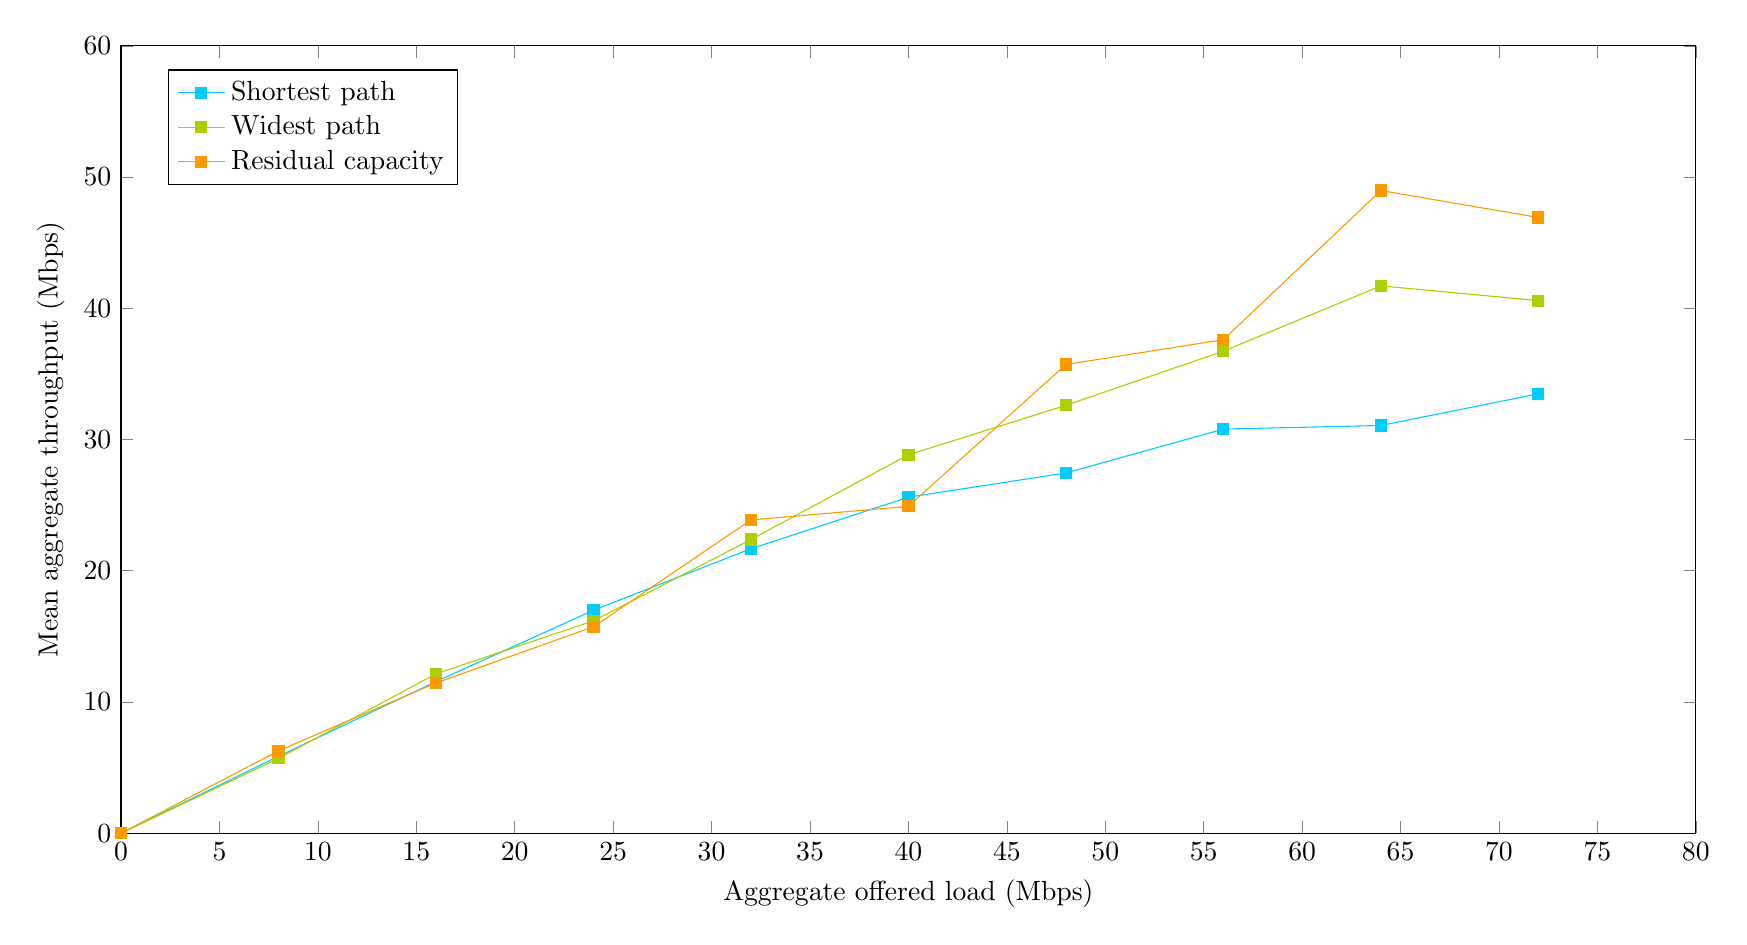
\begin{tikzpicture}
  \begin{axis}[
    width = 20cm,
    height = 10cm,
    xlabel = Aggregate offered load (Mbps),
    ylabel = Mean aggregate throughput (Mbps),
    xmin=0, xmax=80, ymin=0, ymax=60,
    scale only axis,
    legend pos=north west,
    legend cell align=left
  ]

  \addplot[
    mark=square*, mcfblue, draw=mcfblue, 
    %error bars/.cd, y dir=both, y explicit
  ]
  table[x=x,y=y,y error=yerr]
  {
    x       y        yerr
    0 0 0
    8 5.86176695  0.8231965435
    16  11.5535775  1.8500848174
    24  16.9892942  2.7284167978
    32  21.6772777  3.1246555125
    40  25.60601145 4.6067375898
    48  27.4505014  4.268460193
    56  30.79341035 5.1600664391
    64  31.0690037  3.1123100166
    72  33.482466 4.9881937497
  };
  \addlegendentry{Shortest path}

  \addplot[
    mark=square*, mcfgreen, draw=mcfgreen,
    %error bars/.cd, y dir=both, y explicit
  ]
  table[x=x,y=y,y error=yerr]
  {
    x       y        yerr
    0 0 0
    8 5.70097005  0.9819427248
    16  12.1464775  1.959618983
    24  16.1806358  2.8838031317
    32  22.376414 3.157487707
    40  28.836408 4.2771214034
    48  32.6031681  5.1686668287
    56  36.731512 6.2149608988
    64  41.707273 5.0300720744
    72  40.5844955  6.9197951473
  };
  \addlegendentry{Widest path}


  \addplot[
    mark=square*, mcforange, draw=mcforange,
    %error bars/.cd, y dir=both, y explicit
  ]
  table[x=x,y=y,y error=yerr]
  {
    x       y        yerr
    0 0 0
    8 6.2758302105  0.9166252282
    16  11.449755 2.0397464764
    24  15.7299333  2.4486435236
    32  23.8737585  3.6694296596
    40  24.906494 4.0958964659
    48  35.71567985 6.2339491202
    56  37.6072411  5.6730688749
    64  48.971195 5.559440696
    72  46.91598  6.5831520159
  };
  \addlegendentry{Residual capacity}

  \end{axis}
\end{tikzpicture}

\end{document}

\caption{Aggregate throughput comparison for flow pattern `pairs'}
\label{fig:pairs}
Each mark represents the mean of 10 trials for that load/topology combination.
\end{figure}

\begin{figure}
\centering
\documentclass[preview=false]{standalone}

\usepackage{color}
\usepackage{tikz}
\usepackage{pgfplots}
\definecolor{mcfblue}{rgb}{0,0.8,1}
\definecolor{mcforange}{rgb}{1,0.6,0}
\definecolor{mcfgreen}{rgb}{.68,.81,0}
\definecolor{mcfgrey}{gray}{0.95}
\definecolor{mcforange2}{rgb}{1,0.8,0}
\definecolor{mcforange3}{rgb}{1,0.2,0}

\begin{document}

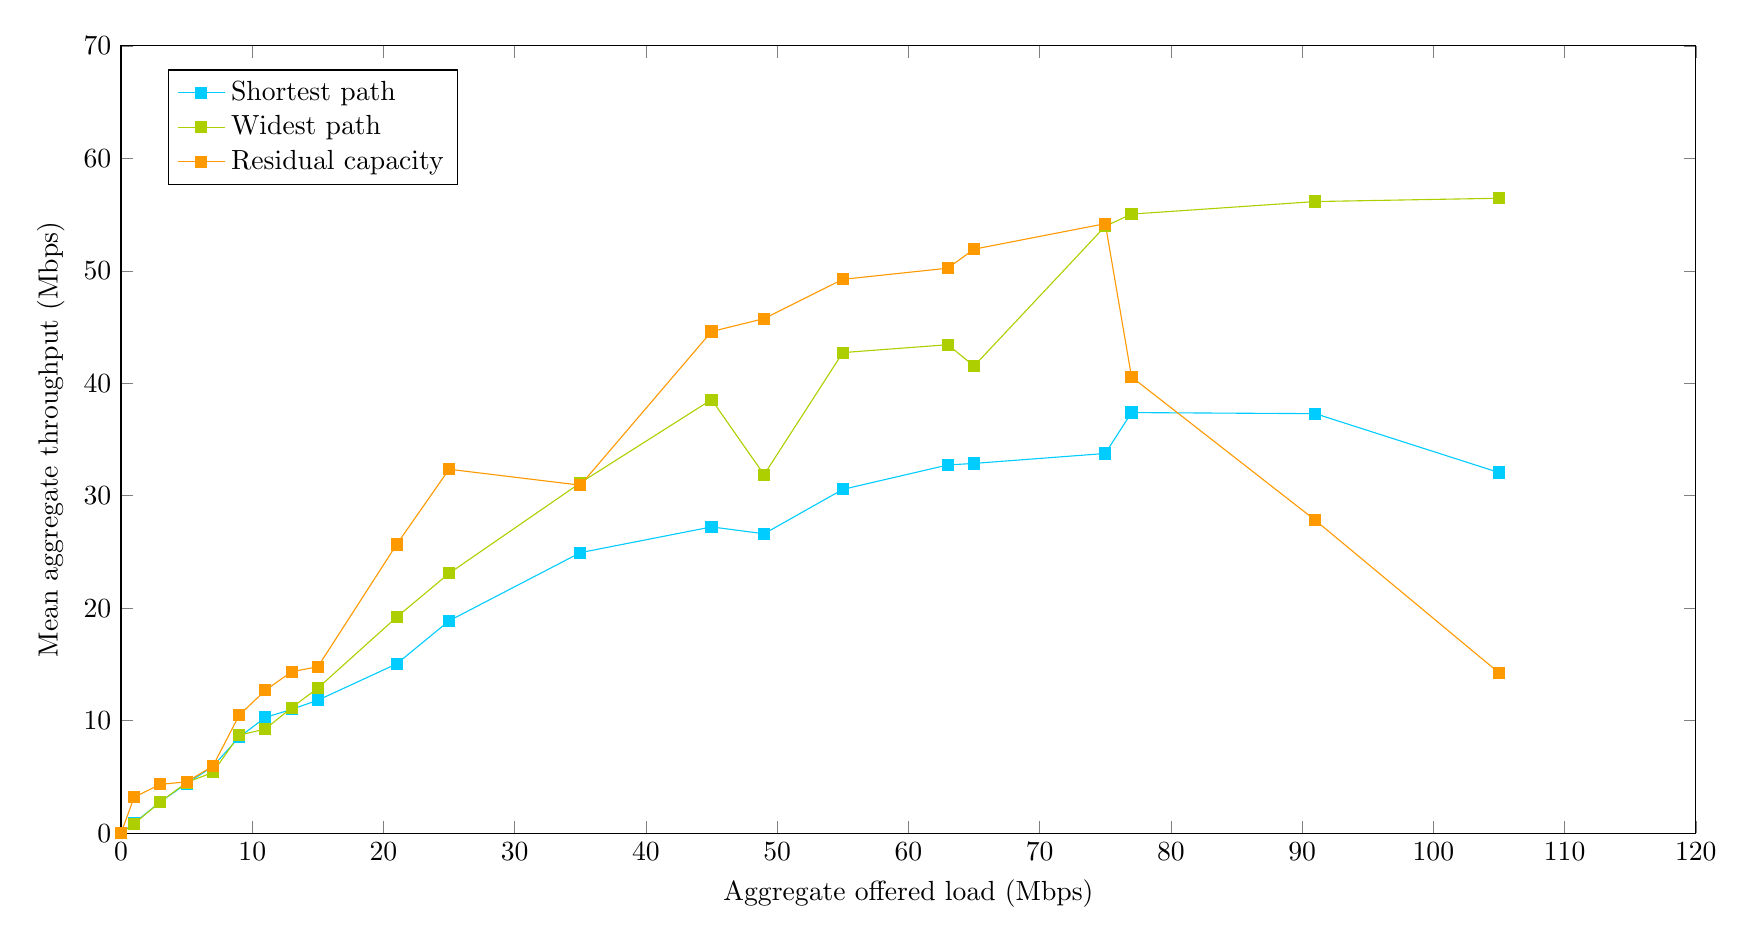
\begin{tikzpicture}
  \begin{axis}[
    width = 20cm,
    height = 10cm,
    xlabel = Aggregate offered load (Mbps),
    ylabel = Mean aggregate throughput (Mbps),
    xmin=0, xmax=120, ymin=0, ymax=70,
    scale only axis,
    legend pos=north west,
    legend cell align=left
  ]

  \addplot[
    mark=square*, mcfblue, draw=mcfblue, 
    %error bars/.cd, y dir=both, y explicit
  ]
  table[x=x,y=y]
  {
    x       y
    0 0
    0 0
    1 0.9076857333
    3 2.7887012
    5 4.4143781667
    7 5.9348530667
    9 8.5344292667
    11  10.2956094667
    13  11.0084661333
    15  11.8237655667
    21  15.0515486667
    25  18.8840666
    35  24.9408325333
    45  27.2294380667
    49  26.6205349333
    55  30.5667652667
    63  32.7360330667
    65  32.8748182667
    75  33.7584818667
    77  37.3938184
    91  37.2973111333
    105 32.0640434
  };
  \addlegendentry{Shortest path}

  \addplot[
    mark=square*, mcfgreen, draw=mcfgreen,
    %error bars/.cd, y dir=both, y explicit
  ]
  table[x=x,y=y]
  {
    x       y
    0 0
    0 0
    1 0.837472
    3 2.7918824
    5 4.5035344333
    7 5.4081212667
    9 8.7153884
    11  9.2621923333
    13  11.1652936667
    15  12.9007854333
    21  19.206016
    25  23.1014973333
    35  31.145868
    45  38.546948
    49  31.8722968
    55  42.7261178
    63  43.4277681333
    65  41.5316588667
    75  53.9628482667
    77  55.0400688667
    91  56.1537334
    105 56.4487925333
  };
  \addlegendentry{Widest path}


  \addplot[
    mark=square*, mcforange, draw=mcforange,
    %error bars/.cd, y dir=both, y explicit
  ]
  table[x=x,y=y]
  {
    x       y
    0 0
    0 0
    1 3.2083705
    3 4.3446018333
    5 4.56657
    7 5.9660251333
    9 10.48575505
    11  12.70449665
    13  14.3583371667
    15  14.7968646667
    21  25.66589895
    25  32.35605065
    35  30.9391424333
    45  44.5982052667
    49  45.7477358
    55  49.2379251333
    63  50.2314286333
    65  51.9199845
    75  54.18844885
    77  40.5596216833
    91  27.82448735
    105 14.2570914833
  };
  \addlegendentry{Residual capacity}

  \end{axis}
\end{tikzpicture}

\end{document}

\caption{Aggregate throughput comparison for flow pattern `random'}
Each mark represents the mean of 15 trials for that load/topology combination.
\label{fig:random}
\end{figure}
\end{landscape}

\section{Scalability of Objective Functions}

\begin{figure}
\centering
\documentclass[preview=false]{standalone}

\usepackage{color}
\usepackage{tikz}
\usepackage{pgfplots}
\definecolor{mcfblue}{rgb}{0,0.8,1}
\definecolor{mcforange}{rgb}{1,0.6,0}
\definecolor{mcfgreen}{rgb}{.68,.81,0}
\definecolor{mcfgrey}{gray}{0.95}

\begin{document}

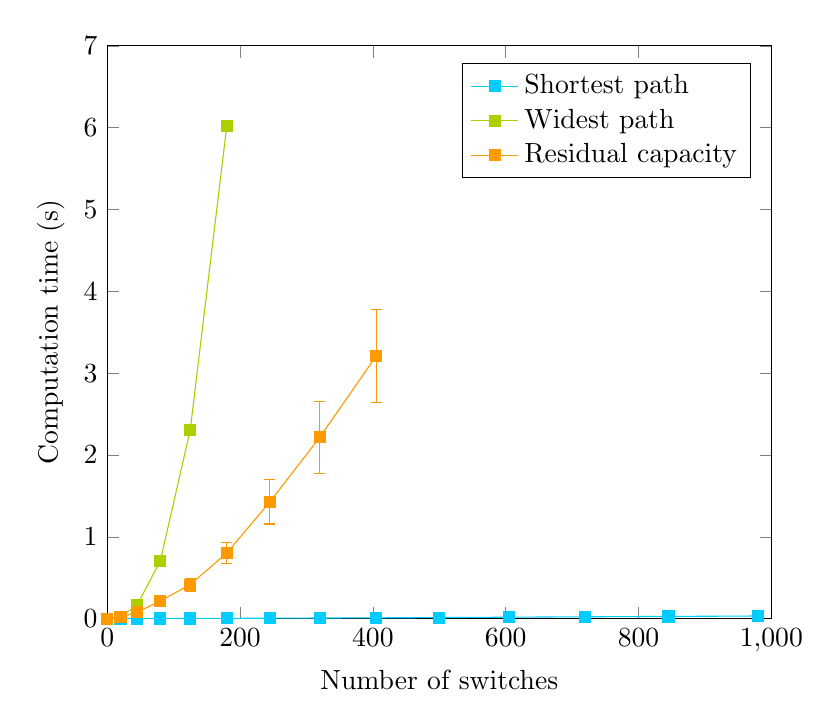
\begin{tikzpicture}
  \begin{axis}[
    xlabel = Number of switches,
    ylabel = Computation time (s),
    xmin=0, xmax=1000, ymin=0, ymax=7,
    scale only axis,
    legend pos=north east,
    legend cell align=left
  ]

  \addplot[
    mark=square*, mcfblue, draw=mcfblue, 
    error bars/.cd, y dir=both, y explicit
  ]
  table[x=x,y=y,x error=xerr,y error=yerr]
  {
    x       xerr    y        yerr
    0 0 0 0
    20  0 0.0004876 1.73519417885663E-005
    45  0 0.0008358 4.18849218990829E-005
    80  0 0.0014721333  6.19053392431026E-005
    125 0 0.0022006 7.2781235901969E-005
    180 0 0.0034614667  0.0001785953
    245 0 0.0051226 0.000218655
    320 0 0.0076167333  0.0002536135
    405 0 0.0097622 0.0004514924
    500 0 0.0126307333  0.0003758768
    605 0 0.0175304667  0.0007970859
    720 0 0.022809  0.0010120146
    845 0 0.0269979333  0.0012781702
    980 0 0.0321096667  0.0015394796
  };
  \addlegendentry{Shortest path}


  \addplot[
    mark=square*, mcfgreen, draw=mcfgreen,
    error bars/.cd, y dir=both, y explicit
  ]
  table[x=x,y=y,x error=xerr,y error=yerr]
  {
    x       xerr    y        yerr
    0 0 0 0
    20  0 0.0227468667  9.30541902746289E-005
    45  0 0.164329  0.0020093485
    80  0 0.706706  0.0081184043
    125 0 2.3045877333  0.0326936456
    180 0 6.0166279333  0.0497968407
  };
  \addlegendentry{Widest path}


  \addplot[
    mark=square*, mcforange, draw=mcforange,
    error bars/.cd, y dir=both, y explicit
  ]
  table[x=x,y=y,x error=xerr,y error=yerr]
  {
    x       xerr    y        yerr
    0 0 0 0
    20  0 0.0194374667  0.0023112736
    45  0 0.0774724667  0.0102995943
    80  0 0.2163074 0.0239292767
    125 0 0.4154031333  0.0805419029
    180 0 0.8022469333  0.1317485442
    245 0 1.4275060667  0.2714548502
    320 0 2.2149086667  0.4411705329
    405 0 3.2092397333  0.5724065512
  };
  \addlegendentry{Residual capacity}

  \end{axis}
\end{tikzpicture}

\end{document}

\caption{Comparison of routing algorithm scalability}
\label{fig:sca1}
Computation time is the time taken to route 16 random flows in Al-Fares fat-tree networks with increasing parameter $k$. Error bars show 95\% confidence intervals but are too small to be visible for the shortest path and widest path metrics. 
\end{figure}

From the perspective of the experiments in this thesis, where the largest network considered was an Al-Fares fat-tree with k=4, the time taken to calculate routes is negligible for all routing metrics.

However, in general an important consideration when selecting a routing metric is the computation time required to calculate routes for all flows in the network. This is particularly important if the objective function is to be rerun every few seconds in order to ensure optimal paths are being used. It is therefore desirable to know how well the objective function scales to larger networks.

Running experiments on Mininet means that there are practical limitations of the system, chiefly availability of RAM, which limit the size of networks which can be emulated with Mininet; this limit is hit long before the scalability of objective functions becomes a factor. However, it is possible to test the scalability of individual objective functions without the surrounding framework, by passing mock network graphs and flow statistics to the function. 

The Al-Fares fat-tree is parametrisable by a parameter $k$, which indicates the number of ports per commodity switch used in the network; this produces a network with $(k/2)^2+k^2$ switches and $k^3/4$ hosts in total, and is therefore easy to scale up to large networks for scalability testing. In this test, flows were randomly generated between 16 random hosts, for Al-Fares networks starting from k = 4 until further tests became impractically slow to run (greater than 5 seconds).  The results of this testing are shown in Figure \ref{fig:sca1}, for each of the three routing metrics.

As expected, the shortest-path metric scales extremely well. The basic algorithm is well-understood, and the particular implementation used here is the one provided with NetworkX, which includes a number of small optimisations as well.

The residual spare capacity implementation is based on the formulation described originally by Walkowiak \cite{walkowiak:residual}. As seen in section \ref{sec:rc}, the performance of the algorithm as a whole depends mostly on the number of possible paths in the network. In its original form, the solution becomes unworkably slow at $k = 6$, with just 45 switches considered. One major optimisation was therefore implemented: the length of possible paths considered is limited to 6 hops. This is enough hops to allow multiple paths to each aggregation and core switch, but not to bounce indefinitely and unnecessarily between the core, aggregation and edge layers. Figure \ref{fig:sca2} demonstrates how much the scalability of the residual capacity metric is dependent on the maximum path length considered.

\begin{figure}
\centering
\documentclass[preview=false]{standalone}

\usepackage{color}
\usepackage{tikz}
\usepackage{pgfplots}
\definecolor{mcfblue}{rgb}{0,0.8,1}
\definecolor{mcforange}{rgb}{1,0.6,0}
\definecolor{mcfgreen}{rgb}{.68,.81,0}
\definecolor{mcfgrey}{gray}{0.95}
\definecolor{mcforange2}{rgb}{1,0.8,0}
\definecolor{mcforange3}{rgb}{1,0.2,0}

\begin{document}

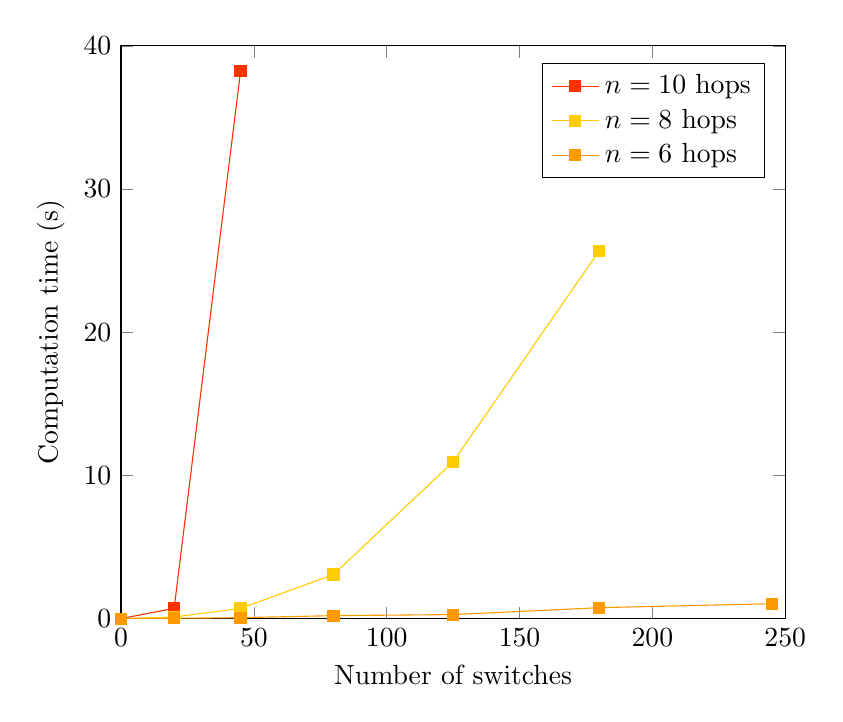
\begin{tikzpicture}
  \begin{axis}[
    xlabel = Number of switches,
    ylabel = Computation time (s),
    xmin=0, xmax=250, ymin=0, ymax=40,
    scale only axis,
    legend pos=north east,
    legend cell align=left
  ]

  \addplot[
    mark=square*, mcforange3, draw=mcforange3, 
    error bars/.cd, y dir=both, y explicit
  ]
  table[x=x,y=y,y error=yerr]
  {
    x       y        yerr
    0 0 0
    20  0.7256292 0.0070739045
    45  38.23024  0.1366292663
  };
  \addlegendentry{$n=10$ hops}

  \addplot[
    mark=square*, mcforange2, draw=mcforange2,
    error bars/.cd, y dir=both, y explicit
  ]
  table[x=x,y=y,y error=yerr]
  {
    x       y        yerr
    0 0 0 
    20  0.1143344 0.0027257511
    45  0.7122406 0.0030605062
    80  3.0836048 0.0217548799
    125 10.9429072  0.011007954
    180 25.692701 0.2385566181
  };
  \addlegendentry{$n=8$ hops}


  \addplot[
    mark=square*, mcforange, draw=mcforange,
    error bars/.cd, y dir=both, y explicit
  ]
  table[x=x,y=y,y error=yerr]
  {
    x       y        yerr
    0 0 0 
    20  0.0277476 0.0003812801
    45  0.06633 0.0036184659
    80  0.2110152 0.005928307
    125 0.283254  0.0053192575
    180 0.7664158 0.0074985986
    245 1.042033  0.0053563215
  };
  \addlegendentry{$n=6$ hops}

  \end{axis}
\end{tikzpicture}

\end{document}

\caption{Effect of maximum path length for residual capacity metric}
\label{fig:sca2}
Computation time is as for Figure \ref{fig:sca1}. Instead of considering all possible paths between hosts, only consider paths with a maximum path length of $n$ hops.
\end{figure}

The widest path metric performs quite poorly for such a well-known routing metric. The algorithm is based on a modified Dijkstra's algorithm, as described in section \ref{sec:wp}, which is not known to be particularly inefficient; the poor performance of the metric in these experiments is likely to be due to poor implementation. In particular, the algorithm must consider every path in the network, so, as for the residual capacity metric, the number of paths in an Al-Fares fat-tree can be very high and this is likely to be a significant factor in the algorithm's scalability. Unlike for residual capacity, however, limiting the number of paths considered was non-trivial due to the particular implementation, so this optimisation was not implemented. However, the dramatic effect of path length on the residual capacity metric seems to indicate that this could provide better scalability in this similar metric as well.

In general, it seems that the approach used in this thesis would be reasonable: route flows initially along the shortest path, then every few seconds, recalculate globally-optimal routes. In a normal scenario, however, the routing recalculation is performed every few seconds, and it is likely that many flows would be similar between calculations. This assumption can be made stronger if flows are consolidated; for example, group `all HTTP traffic' along similar paths instead of calculating flow rules for individual flows, increasing the likelihood that the grouped flow will still be present in the future.

In many optimisation techniques, such as branch-and-bound (used in this work by GLPK \cite{glpk}) and simulated annealing (used in \cite{alfares:hedera}), starting from an estimated solution which is close to the optimum greatly decreases the time taken to reach optimal levels. Here, the previous route allocation could be used as such an estimated solution. However, the implementation of this is non-trivial, and limits the use of third-party interfaces such as PuLP, since there is no way to specify a starting estimate for most solvers. This is far outside the scope of this project and definitely in the realm of `future work'.
